\documentclass[11pt, a4paper, twocolumn]{article}
\usepackage[T1]{fontenc}
\usepackage[utf8]{inputenc}
\usepackage{titlesec}
\usepackage{natbib}
\usepackage{graphicx}
\usepackage{hyperref}
\usepackage{graphicx}
\usepackage[font={small, it}, labelfont=bf, center]{caption}
\usepackage[top=1cm, left=1cm, right=1cm, bottom=2cm]{geometry}

\usepackage{helvet} % Helvetica 'phv'
\usepackage{mathptmx} % Times 'ptm'

\urlstyle{same}

\titleformat{\section}
  {\sffamily\bfseries\Large} % format
  {\thesection} % label
  {1em} % label separation
  {} % before-code

\titleformat{\subsection}
  {\sffamily\bfseries} % format
  {\thesubsection} % label
  {1em} % label separation
  {} % before-code

\title{\sffamily\bfseries DRAFT\\An Exploration of Optimisation Techniques\\for Vulkan-based Particle Systems}
\author{Robin Wragg}
\date{\today}

\begin{document}

\maketitle
%%%%%%%%%%%%%%%%%%%%%%%%%%%%%%%%%%%%%%%%%%%%%%%%%%%%%%%%%%%%%%%%%%%%%%%%%%%%%%%%

\section{Introduction}

The aim of this project is to research and experiment with techniques for optimising the rendering speed of particle systems and Vulkan-based rendering pipelines. The literature is explored and the discovered techniques are applied to our own program, a particle system built in C++ and Vulkan. From this experience, and independent experimentation, we will collect and document the most appropriate techniques.

Multiprocessors will briefly be explored in the literature review, but we will be focussing on consumer-oriented systems with a single, multi-core CPU and a single GPU throughout this paper.

\subsection{Particle Systems}

Various ephemeral phenomena such as fire, rain, explosions and smoke can be challenging to render convincingly and efficiently using the mesh-of-triangles approach that is used for solid objects.

To create an accurate simulation of these phenomena is impossible to do in real-time, because it would require representing many trillions of individual molecules; completely prohibitive from a performance perspective. Particle systems are a way of approximating the behaviour of these systems. The technique involves rendering many emph{particles} per frame; the number of particles is dependant on the intended realism/quality and the required rendering speed. Particle systems are more versatile than just a way to simulate realistic visual effects; they often used to render unrealistic phenomena, such as magical effects.

A particle can be any simple, renderable object; emph{billboards} (flat, textured polygons that always face the camera) are perhaps the most common kind of particle, and can represent an individual droplet of rain or a section of a cloud. But a particle can be anything the framerate allows; full-blown meshes can be used, if the amount and complexity are low enough for real-time rendering.

Particle systems are a useful environment for experimenting with performance because the faster the particles render, the more particles are able to rendered without a noticeable drop in framerate, allowing improved visual results. This quantitative nature makes them appropriate for quantifying the performance impact of any changes made to the program.

\subsection{The Vulkan API}

Vulkan is a cross-platform Application Programming Interface for rendering 3D graphics in real-time. It is developed by the non-profit consortium, the Khronos Group. Along with its contemporaries, Microsoft DirectX 12 and Apple Metal, it was developed to provide a better balance in workload between the CPU and GPU, in response to its precursors, older APIs, namely DirectX 11 and OpenGL, which were often bottlenecked by the single-threaded performance of the CPU.

% TODO: General vulkan pipeline overview; fairly brief and abstract.

\subsection{Multi-threading}

Concurrent execution is the very common technique in modern computing of running multiple threads in a single program; the effect is equivalent to two or more processes with access to the same memory. This allows a CPU with multiple cores to run more than one of these threads at once.

\begin{figure}[h]
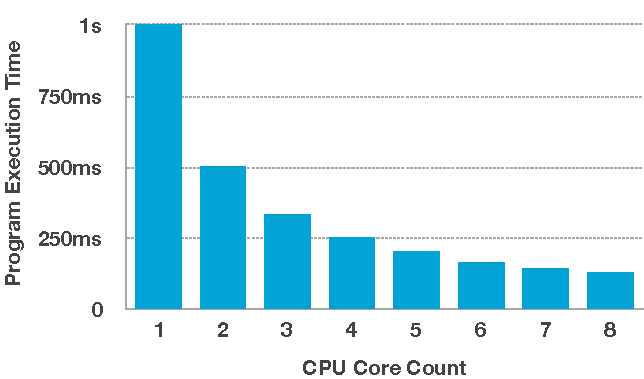
\includegraphics[width=\linewidth]{cpu_cores}
\caption{Theoretical execution time of a program that requires one second of CPU time by core count.}
\label{fig:cpu_cores}
\end{figure}

As it became more difficult for manufacturers to increase the clock speeds of CPU cores, more cores were added instead. Nowadays, all consumer CPUs have at least two physical cores, so the performance of a program can be half of its potential if it doesn't utilise multiple threads effectively in its performance-critical sections. Or inversely, a single-threaded program that requires one second of CPU time can reach a fraction of that time if rewritten as a multi-threaded program, but more cores yield diminishing returns (see Figure \ref{fig:cpu_cores}).


\subsection{Other Topics to Introduce}

If I find that I'm focussing on additional specific areas of research or experimentation, preliminary explanation for those will be written in this subsection.

\section{Literature Review}

\subsection{Performance Profiling}

\subsection{Particle System Design}

% TODO: Current primary particle reference: \cite{Tatarchuk2006} "3.3 Rendering system requirements and constraints" of "artist-directable real-time rain etc" has good info on texture compression, vertex compression. "3.6.2 Raindrop Particles Rain"

\citet{Boulianne2007} implemented a biological system simulator using a 3D grid in which each element can hold one or zero particles. Their simulator needed to take into account the spacial locality of particles; a grid facilitates this by removing the need for distance calculation and particle search. Although their implementation did not have real-time graphics in mind, this grid-based approach could be applied to particle-based rendering for situations where the intended effect requires particles to react to each other based on their proximity. Additionally, ``this system is expected to be suitable for acceleration with parallel customizable hardware,'' \citep{Boulianne2007} meaning this technique would likely be appropriate for rendering real-time particle systems and the parallel nature of GPUs.

When producing a simulation of water droplets on a glass pane... \citet{Chen2012}

\subsection{Techniques for Efficient Real-time Graphics}

\citet{Crawford2018} noted that shader compiler optimisation can make a modest improvement to graphics performance, but it is highly dependent on shader code itself. With their test suite of the LunarGlass/LLVM optimisation framework and the GLSL shaders from GFXBench 4.0, they found that shaders can be sped up by as much as 25\% by finding the best combination of compiler flags, but 1-4\% should be expected in general. Common optimisations that shader compilers can perform are dead code elimination, factoring out conditionals, unrolling loops, coalescing multiple vector element assignments into a single swizzled vector assignment, global value numbering causing variable elimination, and simplifying arithmetic by reordering the statements. The study reviewed only source-to-source optimisations; source-to-machine-code optimisations weren't explored. Further speed-ups could be found in that area.

Referring to Vulkan and DirectX 12, \citet{Joseph2016} states ``the central focus of this new generation of APIs is to increase the amount of draw calls possible while decreasing the amount of overhead for the CPU.'' As graphics programmers, we can reinterpret this to indicate that it is critical to reduce the amount of time that the CPU and GPU are required to block each other to communicate, in order to get the most out of the hardware.

\subsection{Multi-threaded Software Design}

Coordination between threads is a necessary characteristic of reliable multi-threaded systems \citep{Powell}. Without coordination, race conditions and simultaneous unsafe memory accesses can occur, leading to unintended, unpredictable behaviour, often resulting in crashes due to memory access violations. Some ways to avoid these issues are presented below.

\textbf{Mutexes} are perhaps the most common mechanism to ensure thread coordination. A thread can attempt to \emph{lock} a mutex; if the mutex was previously in an unlocked state, the attempt to lock is successful and that thread can continue as normal. The thread now "owns" the mutex. If the mutex is already locked, in most cases the thread will be blocked, and will wait until another thread \emph{unlocks} the mutex (only the owning thread can unlock a mutex). The exception to this is when a \verb|try_lock()| function or equivalent is called on the mutex instead of \verb|lock()|; this will not block the thread, and will instead give the opportunity for the thread to do other work while it waits for  Not all mutex implementation have \verb|try_lock()|, but this functionality is available for this project as part of C++'s \verb|std::mutex| \citep{CppMutex}.

% Paragraph code example
% \begin{verbatim}
% int main() {
%   float a = 3.45;
%   char *str = "oaiwjef";
%   return 0;
% }
% \end{verbatim}

\textbf{Semaphores}

Blocked threads are a significant cause of the reduction of maximum theoretical performance on multi-core systems \citep{Alemany1992}. In the worst case, a \emph{deadlock} can occur when all threads are blocked, waiting on each other indefinitely. In the case of mutexes, a good rule of thumb is to keep the areas of the program that are mutex-guarded as small, simple and fast as possible, to reduce the amount of time that mutexes are locked, thereby reducing the chance of blocked threads.
% TODO: if semaphores have a separate rule of thumb, move this mutex sentence to the mutex detail above and add the semaphore rule of thumb to the semaphore detail.

Although the effects of thread-blocking can be a significant challenge to remove entirely, there exist programming techniques that allow concurrent sections to communicate without blocking each other, such as \emph{exponential backoff}, an algorithm commonly used in network coordination, that slows a process or thread in order to reduce congestion on a shared resource such as an Ethernet node \citep{Goodman2019}, or more applicably for us, a mutex or critical memory. This of course has the downside of one or more threads not operating at their maximum speed but it can have an overall benefit, depending on the bottlenecks of the program.

\emph{Optimistic concurrency control} is another class of algorithms for non-blocking concurrency that involves validating a transaction performed on shared data before committing it \citep{Herlihy1993} in an attempt to detect whether data corruption had occurred due to simultaneous writes or reads. Again, this has a downside of requiring extra work per transaction.

% "" (some of these techniques) are very complex; their usefulness must be weighed against the development team's ability to handle the additional complexity, and the cost of time spent implementing it. For this reason, we began implementing the optimisation techniques that appeared to have a good benefit-to-complexity ratio. % TODO: make a chart of these ratios?

% good structure from "SunOS Multithread Architecture": The remainder of this paper is divided into N sections. The first section gives an overview of the architecture and introduces our terminology. The second section discusses our design goals and principles. The third section gives additional details of operation and interfaces and how the UNIX process model is reinterpreted in the new environment. The fourth section gives some performance data and operational experience. The last section compares this architecture with others.

\section{Initial Approach}

After examining the literature, we decided on a [something] implementation based on the techniques of cite, cite, cite, and cite.

% Intel Core i5 6400
% Nvidia Geforce GTX 1060 3GB
% 8GB ***** RAM


%%%%%%%%%%%%%%%%%%%%%%%%%%%%%%%%%%%%%%%%%%%%%%%%%%%%%%%%%%%%%%%%%%%%%%%%%%%%%%%%
\bibliographystyle{agsm}
\bibliography{mendeley_refs, other_refs}
\end{document}





